\documentclass[11pt,openright,oneside]{report}
\usepackage[utf8]{inputenc}
\usepackage{hyperref} 
\usepackage[portuguese]{babel}
\pagenumbering{arabic}
\usepackage{graphicx}
\usepackage{csquotes}
\usepackage{blindtext}
\usepackage[T1]{fontenc} 
\usepackage{natbib}
\usepackage{minted}


\begin{document}
%%
% Definições
%
\def\titulo{Bases de Dados}
\def\data{3 de Maio de 2015}
\def\autores{Marlene Bastos nº76346, Paulo Gil nº76361}
\def\autorescontactos{marlenebastos@ua.pt, paulogil@ua.pt}
\def\versao{v1.0}
\def\departamento{Departamento de Eletrónica, Telecomunicações e Informática}
\def\empresa{Universidade de Aveiro}
\def\logotipo{ua.pdf}
%
%% CAPA %%
%
\begin{titlepage}

\begin{center}
%
\vspace*{50mm}
%
{\Huge \titulo}\\ 
%
\vspace{10mm}
%
{\Large \empresa}\\
%
\vspace{10mm}
%
{\LARGE \autores}\\ 
%
%
\vspace{30mm}
%
\begin{figure}[h]
\center
\includegraphics{\logotipo}
\end{figure}
%
\vspace{30mm}
\end{center}
%
\begin{flushright}
\versao
\end{flushright}
\end{titlepage}

%
%
%%  Página de Título %%
%
%
\title{%
{\Huge\textbf{\titulo}}\\
{\Large \departamento\\ \empresa}
}
%
\author{%
    \autores \\
    \autorescontactos
}
%
\date{\data}
%
\maketitle

%%%%%%%%%%%%%%%%%%%%%%%%%%%%%%%%%%%%%%%%%%%
% RESUMO
%
%
\pagenumbering{roman}

\begin{abstract}
Neste relatório vai proceder-se à analise detalhada de uma aplicação desenvolvida pelos autores deste relatório. Esta aplicação é um exemplo bastante simplificado de gestão de uma biblioteca comum. 

\end{abstract}

\tableofcontents
\listoffigures

%%%%%%%%%%%%%%%%%%%%%%%%%%%%%%%
\clearpage
\pagenumbering{arabic}

%%%%%%%%%%%%%%%%%%%%%%%%%%%%%%%%

\chapter{Introdução}
\label{chap.introducao}
No âmbito da disciplina de Laboratórios de Informática, foi proposto a relização de um relatório sobre um tema abordado durante as aulas, de forma a consolidar os conhecimentos. Assim sendo, foi escolhido o tema de Base de Dados para que fosse melhor compreendida a utilização e dinâmica desta ferramenta em Python.

Para que este relatório seja compreendido corretamente é necessário a compreensão do que é uma Base de Dados.
As Bases de Dados são fundamentais para as aplicações de hoje em dia pois são como armazéns de informação. Nessas bases está guardado uma quantidade imensa de dados importantes para o funcionamento de outros programas. 
Para a utilização simples das bases tornou-se necessário o desenvolvimento de ferramentas de gestão para a manutenção dos dados. A ferramenta no qual este relatório se foca é a linguagem SQL.

SQL foi desonvolvido nos anos 70 , na IBM* e foi resultado de um projeto que tinha como objetivo mostrar a implementação do modelo relacional*. A sua sigla provém do nome original Structured Query Language**.
Esta linguagem diferencia-se das outras, pois consulta de forma específica o resultado. É portanto uma linguagem declarativa, o que facilita a aprendizagem aos amadores.

Neste relatório vamos apresentar um exemplo de utilização de uma base de dados, integrado com a linguagem Python.

\chapter{Comandos SQL}
\label{chap.comandos}

Para a realização deste relatório foram usados comandos simples: SELECT, UPDATE, INSERT INTO e DELETE.
O comando SELECT é usado para selecionar dados.
Exemplo:

\begin{verbatim}
SELECT * FROM books;
\end{verbatim}
O comando UPDATE é usado para editar registos já existentes numa tabela.
Exemplo:

\begin{verbatim}
UPDATE books SET req = 0 WHERE titulo="O Alquimista";
\end{verbatim}
O comando INSERT INTO é usado para inserir novos registos numa tabela.
Exemplo:

\begin{verbatim}
INSERT INTO users VALUES (null,'Paulo Gil','paulogil@ua.pt','925007392');
\end{verbatim}
O comando DELETE é usado para eliminar registos numa tabela.
Exemplo:

\begin{verbatim}
DELETE FROM requisitions WHERE book="Marley e Eu";
\end{verbatim}

\chapter{Descrição do programa}
\label{chap.descricao}

O problema sugerido para a consolidação de conhecimentos consistia numa gestão de uma biblioteca. O funcionamento de uma biblioteca baseia-se no registo de requisições feitas pelos seus utilizadores e na manutenção dos livros e utilizadores.

Para isso, foi criada uma base de dados, através da ferramenta SQLite, contendo 3 tabelas. A primeira, chamada de books, serve para guardar os registos dos livros existentes na biblioteca. Tem como colunas o título do livro, o autor, e uma chave tomando os valores de zero ou um. Esta chave serve para verificar se o livro está requisitado ou não: zero para não requisitado; um para requisitado.
	
A outra tabela, chamada de users, tem como finalidade a gestão dos utilizadores da biblioteca. Informações como o nome, o email e o contacto, são guardados nas colunas desta tabela.

Por fim, a tabela requisitions gere todas as requisições efetuadas pelos utilizadores. O título do livro, o utilizador que o requisitou, a data da requisição e a data limite de entrega são campos que preenchem as colunas desta tabela.

\chapter{Apresentação do programa}
\label{chap.apresentacao}

O programa baseia-se em menus estruturados através de funções, no qual são chamadas na função main.

Para dar um certo dinamismo, foi criada uma função chamada cls(), cuja funcionalidade é limpar o ecrã da linha de comandos. Esta função é chamada, sempre que uma nova página do menu entra em ação.

\begin{minted}[frame=lines,fontsize=\footnotesize,linenos]{python}

import os

def cls():
	os.system(['clear','cls'][os.name == 'nt'])

\end{minted}

As principais funções da aplicação são a procura de livros, por título, autor e até por estado da requisição, listar utilizadores e requisições, criar e eliminar livros ou utilizadores.

Um dos aspectos a notar da aplicação e que foi pensado durante o seu desenvolvimento é que quando se elimina um livro ou até mesmo um utilizador, tem um certo valor lógico remover também a sua requisição.


\chapter{Testes funcionais}
\label{chap.testes}

\begin{figure}[!h]
\centering
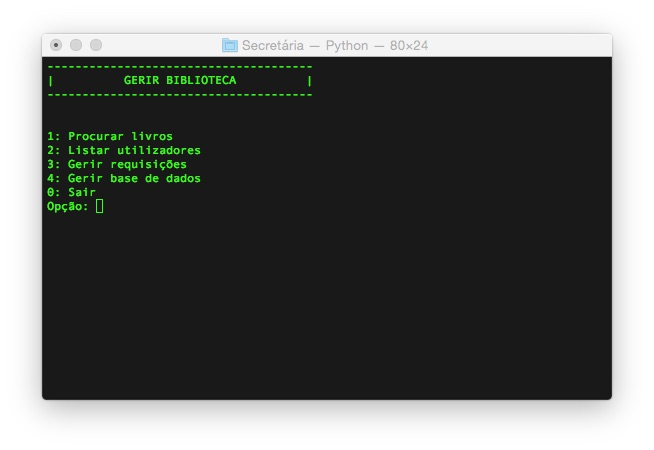
\includegraphics[scale=0.5]{menu_principal.jpg}
\caption{Menu principal}
\end{figure}

\begin{figure}[!h]
\centering
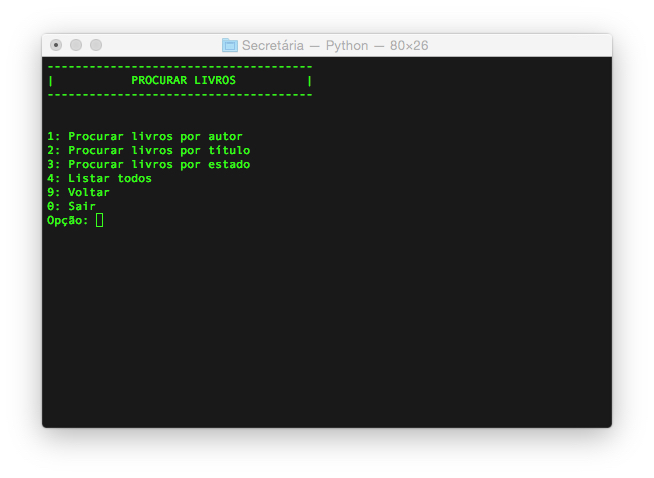
\includegraphics[scale=0.5]{menu_procurar_livros.jpg}
\caption{Menu de procura de livros}
\end{figure}

\begin{figure}[!h]
\centering
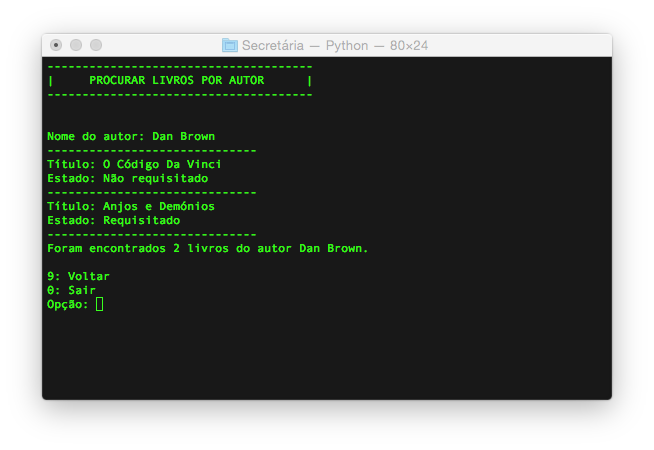
\includegraphics[scale=0.5]{procurar_livro_autor.png}
\caption{Procurar livros por autor}
\end{figure}

\begin{figure}[!h]
\centering
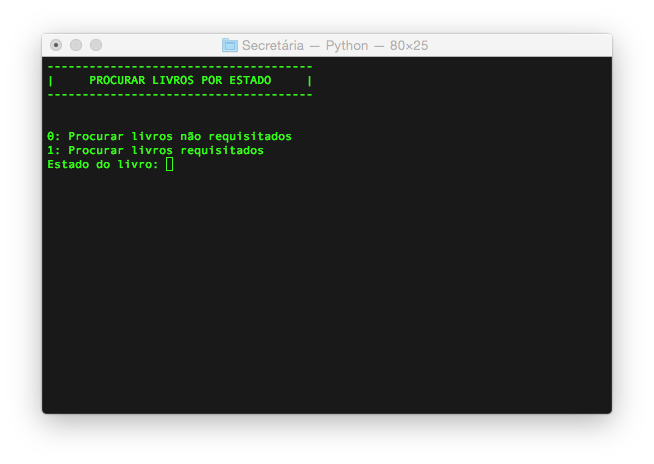
\includegraphics[scale=0.5]{procurar_livros_estado.jpg}
\caption{Procurar livros por estado}
\end{figure}

\begin{figure}[!h]
\centering
\includegraphics[scale=0.5]{fazer_requisicao.jpg}
\caption{Menu de requisições}
\end{figure}

\begin{figure}[!h]
\centering
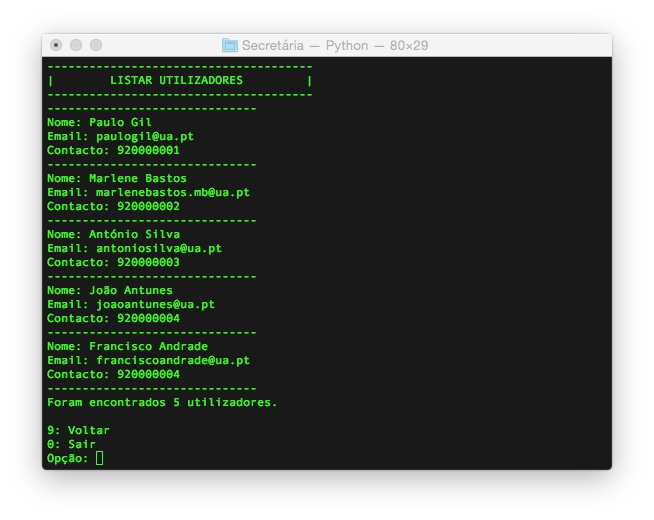
\includegraphics[scale=0.5]{listar_utilizadores.jpg}
\caption{Listar utilizadores}
\end{figure}

\begin{figure}[!h]
\centering
\includegraphics[scale=0.5]{requisicoes.jpg}
\caption{Livros requisitados}
\end{figure}

\begin{figure}[!h]
\centering
\includegraphics[scale=0.5]{fazer_requisicao.jpg}
\caption{Fazer requisição}
\end{figure}

\begin{figure}[!h]
\centering
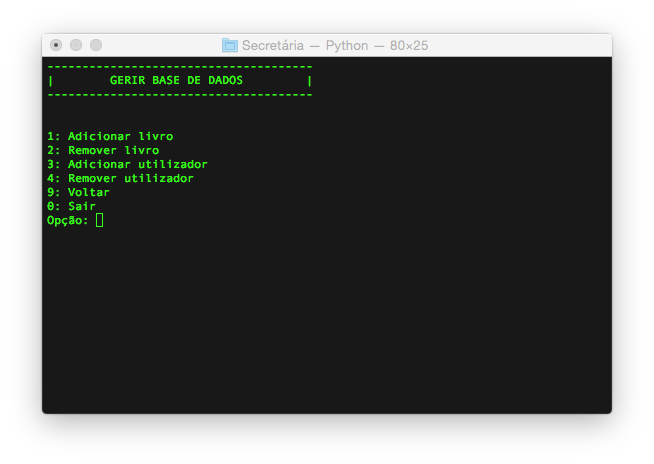
\includegraphics[scale=0.5]{gerir_base_dados.png}
\caption{Menu de gestão de base de dados}
\end{figure}

\chapter{Conclusão}
\label{chap.conclusao}

Com este relatório e após a implementação e gestão de uma base de dados em SQL, conclui-se que é uma ferramenta indispensável no mundo da programação.
A facilidade de integração com outras linguagem, neste caso Python, faz com que seja muito simples de gerir qualquer tipo de dados de uma forma muito rápida e eficiente.
Numa versão futura poderia ser melhorado o sistema de menus, de forma a que fosse escolhido o livro requisitado atráves de um input do teclado e também um sistema que avisasse quais os livros que já deviam ter sido entregues.

\nocite{*}
\bibliography{bibliografia}
\bibliographystyle{plain}

%%%%%%%%%%%%%%%%%%%%%%%%%%%%%%%%%

\end{document}